%     1.3.1. Ingeniería de proteínas
%         1.3.1.1. Ingeniería de proteínas modulares (a.k.a. quiméricas) (Qué es, 1 página)
%         1.3.1.2. Ejemplos (1 página y 1 figura)
%     1.3.2. Ingeniería de linkers.
%         1.3.2.1. Diseño positivo (propiedades deseadas, 1 página, 1 figura)
%             1.3.2.1.1. Propiedades conformacionales
%             1.3.2.1.2. Carga
%         1.3.2.2. Diseño negativo (propiedades no deseadas, 2 páginas y 1 figura)
%             1.3.2.1.1. Propiedades conformacionales
%             1.3.2.1.2. Propiedades espectroscópicas
%             1.3.2.1.3. Actividades biológicas
%             1.3.2.1.4. Carga metabólica
%         1.3.2.3. Linkers naturales
%             1.3.2.3.1 Características (1 página y 1 figura)
%             1.3.2.3.2 Uso en ingeniería de proteínas (ventajas y desventajas, 1 página)
%         1.3.2.4. Diseño racional
%             1.3.2.4.1 Diseños y conceptos comunes (1 página y 1 figura)
%             1.3.2.4.2 Algoritmos existentes (cómo funcionan, ventajas y desventajas, 2 páginas y 2 figuras)
%             
       
\section{Ingeniería de proteínas}\label{proteinEngineering}
\subsection{Ingeniería de proteínas modulares}    

Como producto de los avances logrados en las tecnologías asociadas al ADN recombinante, se ha desarrollado una nueva generación de proteínas compuestas por la integración
de diferentes módulos secuenciales.

La idea de armar proteínas a partir de la unión de módulos no es algo nuevo, sino que sigue la lógica presentada previamente de que las proteínas naturales son usualmente modulares. 
Es decir, se está simulando el proceso evolutivo natural que desarrolla nuevas proteínas mediante la combinación de dominios preexistentes.

La utilización de la técnica de ADN recombinante para construir nuevas proteínas abre toda una gama de posibilidades que van desde inserción de pequeñas secuencias en extremos de proteína naturales, 
con el fin de poder identificarlas o separarlas, hasta el diseño de construcciones proteicas que buscan obtener nuevas funcionalidades o propiedades diferentes.
% construidas mediante la combinación de distintos dominios.
% En los casos más simples el proceso puede ser ...
% En el caso de nuevos diseños, donde se busca combinar módulos para dar nuevas funcionalidades o hacerlas más eficientes, el proceso experimental puede ser mas complejo.

% s primeros ejemplos de construcciones artificiales probablemente sean la inserción de epítopes o tags(pequeñas secuencias?) en los extremos de alguna proteína para poder localizarlas y/o separarlas.
% en solución o en el entorno celular.
% Más adelante se desarrollaron nuevas construcciones combinando unidades estructurales y/o funcionales en una sola molécula. 
% Esta fusión de dos o más dominios abre toda una gama de posibilidades para construir proteínas con nuevas o mejores funcionalidades.
% 

% Las distintas bases de datos permiten obtener, entonces, una gran cantidad de módulos estructurales y funcionales y gran parte del diseño de proteínas quiméricas 
% se basa en utilizar estos conocimientos y anotaciones para crear nuevas proteínas con estructuras/funciones/propiedades combinadas.

En estos últimos casos, la implementación del proceso experimental suele ser más complejo, requiriendo varios aspectos de diseño a considerar, los 
los cuales no siempre son totalmente independientes entre si. 
% requiriendo un diseño   o un proceso iterativo.
Por un lado está el proceso de diseño/construcción de la nueva proteína.
Por otro están los aspectos asociados con la técnica de ADN recombinante y expresión de proteinas heterólogas. 
En el gráfico \ref{esquemaProcesoFusion} se representan los pasos generales que pueden formar parte de este proceso.

\begin{figure}[htbp]
\centering
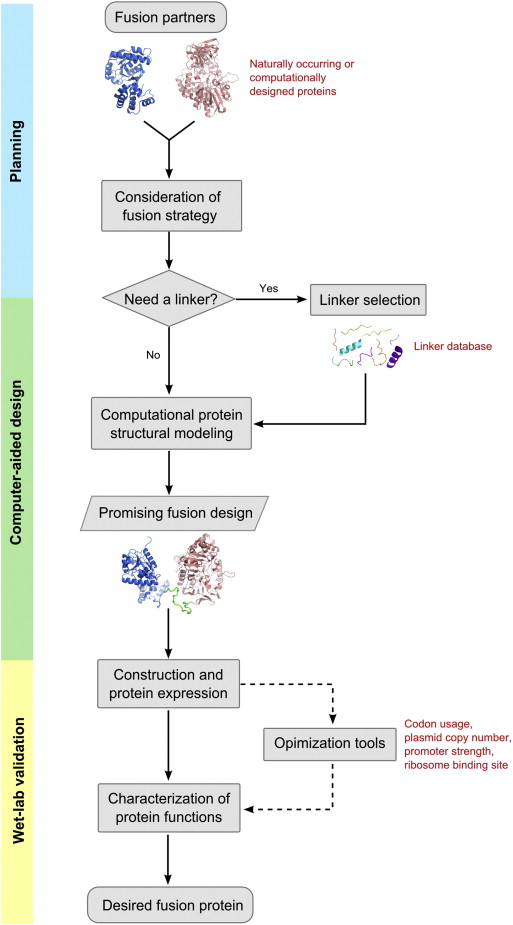
\includegraphics[width=0.7\textwidth]{img/esquemaProcesoFusion.jpg} 
\caption{Figura obtenida de \cite{yu2015synthetic}}
\label{esquemaProcesoFusion}
\end{figure}

La construcción de la proteína de fusión(quimérica) requiere, por su parte, de dos elementos indispensables: 
los dominios o proteínas a fusionar, y la secuencia linker que los va a unir.
La elección de los dominios/proteínas está fuertemente ligada al producto final que se desea obtener y, normalmente, es una decisión directa alrededor de la cual se diseña el resto del experimento.
Por otro lado, la selección de un linker adecuado para unir los dominios/proteinas de acuerdo al objetivo que se busca puede ser un paso complicado y es generalmente ignorado cuando se piensa en el diseño de una proteína quimérica.
La unión directa de los dominios/proteínas o el uso de un linker inadecuado puede resultar en resultados indeseables, por ej. puede restringirse la capacidad de plegado de algun dominio globular, 
bajar el rendimiento de la proteína resultante o disminuir en la actividad biológica de alguno de los módulos.
La correcta selección, o mejor aún, el diseño racional de las secuencias linker para unir los módulos es un aspecto importante, aunque poco desarrollado, del diseño de proteínas quiméricas. 
Esta falta de desarrollo en el tema se debe, quizás, a la falta de conocimiento sobre los factores estructurales que gobiernan la flexibilidad entre los dominios, y es un factor claramente 
limitante en el diseño \textit{de-novo} de proteínas quiméricas. 
Los conocimientos relevantes sobre este tema pueden aparecer a partir de la gran cantidad de secuencias que se disponen actualmente, los avances en 
la identificación de dominios y nuevas técnicas para obtener sus propiedades conformacionales a partir de la información secuencial.





% EJEMPLOS

%

% Examples of this approach include green fluores-
% cent protein (GFP) 1 fusion proteins used in cellular localiza-
% tion studies (1), new antibody types such as multivalent
% antibodies and single-chain antibodies (2-7), artificial
% restriction enzymes consisting of zinc-finger and nuclease
% domains (8, 9),





% AGREGAR ALGO DE TECNICAS FRET
\begin{itemize}
 \item Creación de proteinas que combinan funciones de distintos dominios:
Cómo se dijo en la sección anterior, se poseen cada vez mas dominios anotados con una gran cantidad de funciones correspondientes.
La forma mas común de crear proteinas quiméricas es, entonces, fusionar genéticamente dos o más dominios con subfunciones distintas, obteniendo una nueva funcionalidad global para la proteína.
\item Facilitar el estudio de interacciones proteina-proteina\cite{reddy2013linkers}: 
Tradicionamlente el estudio se hace expresando conjuntamente las dos proteinas que conforman el complejo.
Sin embargo, si la afinidad es muy baja, no es tan simple obtener el complejo formado.
La creación de una proteína quimérica que une a los dominios/proteínas que forman el complejo permite mantenerlas unidas mediante un linker.
La flexibilidad de esta secuencia linker debería permitir la correcta formación del complejo y, al estar unidas covalentemente, habrá una posibilidad mucho mayor de interacción.
El aumento en la estabilidad del complejo permite realizar los estudios biofísicos necesarios sobre éste.
% The characterization of protein–protein interactions is often required to gain an understanding of various biological processes. 
% Yet, the study of protein–protein interactions for many complexes is hampered when one or more partners of the complex are unfolded or unstable. 
% Traditionally, this problem has been addressed by the co-expression and/or copurification of both proteins. 
% However, for weakly interacting or unstable complexes, the co-expression and/or co-purification often results in a single pro-
% tein. 
% Protein engineering techniques were another
% option to address unfolded or unstable proteins,
% using a single polypeptide chain chimera to link the
% two binding partners via a flexible amino acid linker
% 13
% . With these chimeric proteins, it was then possible
% to maintain both the intramolecular and intermolec-
% ular protein–protein interactions, 14 and chimeric
% proteins have been used to generate stable, soluble
% binary complexes for structural studies, as well as
% functional dimers.
% Linking binding partners using an artificial
% linker will increase the proximity between the inter-
% acting partners and preserve the natural interaction.
% In cases where the interacting partners are not
% linked, it is possible that the binding partners might
% dissociate due to their low affinity and/or due to the
% crystallization conditions.
\item La unión de fragmentos de anticuerpos a enzimas o proteínas que permitan la detección de la unión es la base de las técnicas inmunoquímicas.
% \item Incrementar la expresión de proteínas.
\item La unión de segmentos de secuencia específica permite la purificación de proteínas a partir del lisado celular. 
% Facilitar la purificación de proteínas.
% Una de las aplicaciones mas interesantes es para ayudar al estudio estructurals de las intereacciones entre proteinas \cite{}.
% -In addition to structural studies of protein–protein interactions \cite{reddy2013linkers}.,
% \item a wide range of applications in the field of biotechnology have employed these fused proteins
% \item to explore protein-based biochemistry, such as to create artificial bifunctional enzymes and as tools for FRET analysis.

% They have also been widely applied for drug targeting, since proteins such as single chain antibodies or ligands for cell surface receptors can 
% specifically target a linked functional protein (e.g. toxin or cytokine) to a specific type of cells
\end{itemize}












\subsection{Ingeniería de secuencias linker}

% EN ESTA  SECCION PONER LA LISTA COMPLETA DE LOS REQUERIMIENTOS POSITIVOS Y NEGATIVOS DE UN LINKER:
% LONGITUD, COMPOSICION, CONFORMACION DESORDENADA INTRINSECA, AUSENCIA DE ESTRUCTURA SECUNDARIA, AUSENCIA DE ELEMENTOS FUNCIONALES

% \subsubsection{Diseño positivo}


A la hora de obtener un linker las propiedades estructurales suelen ser las más criticas. 
Mantener los dominios unidos a la vez que estos actúan como unidades independientes(manteniendo su funcionalidad), permitiendo que se muevan libremente y la posibilidad de cualquier interacción entre ellos.
Esto depende directamente de la longitud y conformación adoptada por la secuencia linker. 
La longitud no suele ser una propiedad determinante, permitiendo un amplio rango de longitudes efectivas siempre que se eviten las secuencias muy cortas que no permiten una separación suficiente, 
o las secuencias extremadamente largas que harían casi inperceptible la unión de los dominios.
% harían muy ineficaz la interacción entre proteínas.

Los requerimientos conformacionales son un poco mas estrictos y pequeños cambios en la estructura pueden limitar la funcionalidad del nuevo diseño.
En primer lugar buscamos que la secuencia adopte una conformación intrínsecamente desordenada, la cual evita que       manteniendo la
Esta conformación intrínsecamente desordenada provee, además, la flexibilidad necesaria para que los dominios se muevan libremente explorando distintas conformaciones globales.
Para las arquitecturas más comunes, compuestas de dominios globulares unidos por linkers, esta flexibilidad es el requerimiento mas importante ya que permite a los distintos dominios interaccionar libremente.

En la figura \ref{conformacionLinker} se muestran como influyen estos requerimientos en la construcción de una proteína quimérica que une dos dominios EBFP y EGFP. 
Los gráficos A,B y E muestran conformaciones globales de la proteína que son posibles gracias a la flexibilidad del linker intrínsecamente desordenado y con una longitud apropiada. 
Las interacciones que permiten estas conformaciones no se pueden obtener cuando se usa una secuencia con estructura de estructura de hélice-$\alpha$ como se ve en las figuras C y D, donde la rigidez de ésta estructura 
hace que las conformaciones globales sean mucho más limitadas.


\begin{figure}[htbp]
\centering
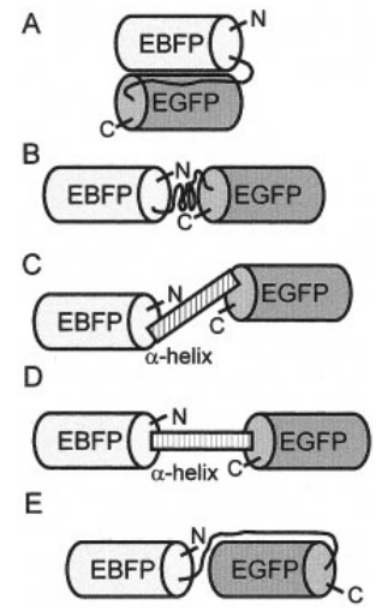
\includegraphics[width=0.3\textwidth]{img/conformacionLinker.png} 
\caption{Figura obtenida de \cite{arai2004conformations}}
\label{conformacionLinker}
\end{figure}


% como vimos antes, el proceso experimental asociado a obtener una proteína quimérica tiene varios pasos, y es importante que la etapa de diseño no se piense en la funcionalidad de la construccion(proteina) 
% de forma aislada sino que se tengan en cuenta las distintas técnicas que pueden/deben utilizarse durante el proceso y en los diferentes contextos donde la proteína se encontrará y donde deberá mantener sus propiedades.

El objetivo de la proteína es poder expresarla en un sistema biológico donde cumplira la función para la cual fue diseñada, por lo tanto es importante que las
propiedades conformacionales del linker se mantengan ante la presencia de otras proteínas o cualquier tipo de ligando.
% MOREs  y Agregacion




% Actividad biologica
La idea del diseño uniendo distintos módulos es que la funcionalidad global se origine exclusivamente a partir de la unión de éstos, por lo tanto la secuencia que los une no debe proveer ninguna funcionalidad adicional, es decir,
debe permanecer inerte ante el entorno en el cual la nueva proteína desarrolla su actividad. 
Las actividades biológicas pueden ser muy variadas pero   
Dado que las propiedades conformacionales  
Entre las actividades biológicas asociadas a estos segmentos están las modificaciones post-traduccionales, unión a ligandos, sitios de clivaje, etc.
Por lo tanto, es importante que la secuencia linker este libre de cualquier funcionalidad asociada a patrones secuenciales lineales. 






% 
% Los requerimientos en el linker no están limitados a la función o actividad de la proteína resultante. 
% Como se vió en la sección anterior, el proceso de 
% 


% COMPOSICION DE AMINOACIDOS: Carga metabolica y propiedades espectroscópicas
% Existen aspectos importantes a la hora de diseñar un linker que podrían parecer obvios, la composición y la longitud del linker son los primeros aspectos a considerar\cite{robinson1998optimizing}.



Por otro lado, la carga de la secuencia puede mediar interacciones en el entorno celular, por ejemplo, al construir proteínas cuya función requiera unirse al DNA es 
requerir que la secuencia linker no tenga residos carga ya que 

Otros requerimientos pueden no aparecer a partir de patrones secuenciales sino de propiedades intrínsecas de cada aminoácido. 
De esta forma, algunos requerimientos están relacionados con la composición secuencial. 
% CARGA METABOLICA
Un ejemplo claro de esto está en poder regular la carga metabólica asociada a la expresión de la secuencia linker. 
Dado que la proteína diseñada deberá ser, finalmente, expresada en algún sistema biológico, y que los distintos aminoácidos que conforman las proteínas tienen distintos costos metabólicos asociados, 
poder controlar la composición(imponiendo una menor frecuencia a aquellos aminoácidos con mas costo metabólico) permitiría incrementar el nivel expresión de la construcción creada.

% propiedades espectroscópicas
En otros casos, el requerimiento está asociado con propiedades fisicoquímicas de algunos aminoácidos. 
Por ejemplo, dado que las dado que las técnicas espectroscópicas se usan de forma rutinaria en el trabajo con proteínas, es deseable que el linker resultante tenga una composición específica tal que no posea aminoácidos que absorban en rango 
del UV, de forma que se elimine cualquier interferencia de la secuencia en este tipo de técnicas.

Otro ejemplo que afecta a la composición está asociada con interacciones iónicas no deseadas. 
Por ejemplo al construir una proteína cuya funcionalidad esté asociada a la unión a DNA, será deseable que la composición final no contenga aminoácidos que puedan encontrarse en estados con carga positiva, debido a que 
la formación de interacciones con la estructura de fosfatos propia del DNA podría interferir en la función de la proteína.

Teniendo en cuenta estos aspectos, una ventaja importante del proceso de diseño es poder definir la composición de la secuencia resultante.


% carga neta
% RESIDUOS CARGADOS
% Una ventaja importante del proceso de diseño es que se pueda definir la carga neta que tendrá la secuencia linker. 
% Este requerimiento puede tener varios fundamentos, principalmente 
Distintas técnicas de laboratorio para identificación y purificación de proteínas se basan en la carga neta de la secuencia.




% Esto se traduce en dos propiedades de la secuencia: que adopte una conformación extendida evitando que los dominios se compacten en el sitio de unión a través del linker, y que no posea una tendencia a adoptar estructuras secundarias, 
% ya que estas podrían reducir el número y tipo de interacciones posibles entre los dominios.


% Es relevante aclarar acá que, si bien los terminos desordenado y flexible pueden solaparse en algun punto, son términos distintos\cite{radivojac2004protein}
% Para una proteína plegada, la flexibilidad refiere a la desviación de las posiciones atómicas con respecto a la estructura promedio en equilibrio.
% Para una region desordenada, la variación en la flexibilidad se refiere a las diferencias en las velocidades de interconversión entre los diferentes estados miembro del ensamble estructural.
% Una variedad de técnicas biofísicas, como por ej. NMR, han sido usadas para estudiar estos conceptos de flexibilidad.

% Análisis de estructuras mediante estas tecnicas muestran que el movimiento en la proteína que provoca los cambios conformacionales puede ocurrir tanto a nivel de residuos como a nivel de estructura secundaria o terciaria. 


% Control of structural flexibility is essential for the proper functioning of a large number of proteins and multiprotein complexes. 
% At the residue level, such flexibility occurs due to local relaxation of peptide bond angles whose cumulative effect may result in large 
% changes in the secondary, tertiary or quaternary structures of protein molecules. 
% Such flexibility, and its absence, most often depends on the nature of interdomain linkages formed by oligopeptides.


% residues or at the secondary, tertiary, or quaternary structural levels. 
% Lactate dehydrogenase, triose-phosphate isomerase, as well as hemoglobin 
% and related proteins are some of the earliest examples of proteins that showed conformational changes with important functional implications.

% 



% 
% 
% 
% 
% La arquitectura típica creada, representada por dominios globulares unidos por secuencias linkers, busca que éstos permitan 
% mantener los dominios separados a la vez que se les da suficiente capacidad para moverse libremente como parte de su funcionalidad. 
% Por lo tanto, la flexibilidad es el requerimiento mas importante, y es deseable que un linker tenga tendencia intrínseca a adoptar una conformación extendida.
% Es importante que, como parte del diseño de la secuencia linker, se asegure que codifique una conformación intrínsecamente desordenada que no posea las características de una estructura colapsada propia de proteínas globulares.
% La conformación extendida le provee la flexibilidad global necesaria, a partir de la rápida interconversión entre la gran cantidad de conformaciones del ensamble con valores de energía similares.
% 
% 
% Un requerimiento asociado 
% Asociado a esto está la idea que una propiedad altamente desfavorable para el linker es que tenga cierta tendencia a adoptar estructuras de hojas-$\beta$ o helice-$\alpha$, ya que los angulos de torsion están limitados al rango
% impuesto por esta estructura, lo que podría también limitar la flexibilidad.
% Como vimos en las secciones previas, 
% aún cuando estas no se encuentren en una conformación plegada compacta típica de proteínas globulares.
% 



% SIGO CON EL EJEMPLO DE FRET QUE HAY MUCHA INFORMACION Y GRAFICOS INTERESANTES
% el ejemplo de FRET permite ejemplificar los requerimientos conformacionales, principalmente de flexibilidad. 
% En este caso, 
% Dado que, la funcionalidad resultante de la proteína quimérica creada depende completamente de la capacidad que 
% 







% % % % % % % ESTO LO PUEDO PASAR A LA PARTE DE LINKERS EMPIRICOS
% 
% % ACA EMPIEZO A HABLAR DE OTROS ASPECTOS NO ESTRUCTURALES
% Sin embargo, la flexibilidad no es todo.  
% Por ej. una opción evidente seria usar linkers de solo Glicina ¿Por qué no usar siempre un linker puramente poli-G, adaptando solamente su longitud?
% Desde los primeros estudios sobre linkers naturales \cite{argos1990investigation} se encontró que las proteinas naturales no usan(seleccionan) este tipo de secuencias.
% Si bien esto no es concluyente para que no se usen, puede darnos un motivo para pensarlo dos veces.
% En primer lugar, un péptido poli-G sería extremadamente inestable y por lo tanto podría actuar como una carga energética, estructural o interferir en procesos de catálisis de los dominios que une, 
% especialmente si tiene una longitud excesiva.
% Se conoce además que el patrón Gly-Gly-X, donde X es un residuo con cadena lateral hidrofóbica, es un sitio target de actividad proteolítica. 
% Por otro lado, una secuencia nucleotídica con alto contenido de Guanina(el codón que codifica para Glicina contiene Guanina en 2 de las 3 posiciones) puede ser difícil de manejar experimentalmente y de expresar para el huésped.
% Como se ve, entonces, existe una gran variedad de aspectos a considerar que exigen distintos requerimientos además de las propiedades conformacionales.
% Por ejemplo, es importante que los linkers should be invulnerable to host proteases, as they are often the targets for degradation. 
% 
% 
% El linker poli-G es sólo un ejemplo. 
% Como vimos en secciones anteriores, distintos elementos funcionales(que actuan principalmente mediante mecanismos de reconocimiento) pueden encontrarse en regiones con distintas propiedades conformacionales. 
% La existencia de estos elementos debe tenerse en cuenta cuando se esta usando la secuencia linker diseñada, y/o su eliminación debe formar parte de la etapa de diseño del linker.
% La longitud del \textit{loop} creado por el linker puede tener un profundo efecto sobre la actividad del linker en una proteína quimérica\cite{nagi1997inverse}.
% Además del ejemplo simple de resistencia proteolítica, las regiones linker también pueden afectar la estabilidad, solubilidad, formación de complejos.
% linker regions can affect the stability, solubility, oligomeric state, and proteolytic resistance ofthe fused protein
% Como se muestra en \cite{robinson1998optimizing}, en algunos casos se tienen efectos importantes variando la longitud y composición de la secuencia
% En base a esto, es esperable que se tengan requerimientos específicos relacionadas con la longitud y la composición. 
% % The stable linkage between functional domains provides many advantages such as a prolonged plasma half-life (e.g. albumin or Fc-fusions). 
% % However, it also has several potential drawbacks including steric hindrance between functional domains, decreased bioactivity, and altered biodistribution and metabolism of the protein moieties due to the interference between domains 
% % In other systems, however, linker regions can affect the stability, solubility, oligomeric state, and proteolytic resistance of the fused proteins
% % Thus, it is important that the length and amino acid composition of a potential linker is optimized in order to preserve the biological activity of the individual proteins in the fused complex.
% 
% 





% \subsubsection{Diseño negativo}




% Además de los analisis sobre las propiedades físicas asociadas a las arquitecturas modulares, el estudio de la diversidad de linkers
% encontrados en la naturaleza puede proveer información importante para entender los requerimientos
% más importantes en el diseño de estas secuencias.


\subsubsection{Linkers naturales}



% 


% El 'descubrimiento' de las regiones/secuencias linkers esta ligado a las teorias de structura-funcion(desarrolladas en la parte de conformacion) que se dieron durante casi 100 años
% En un principio se comenzo a pensar en una estructura rigida asociada a la proteina, luego se fueron revelendo propiedades dinamicas que le permitian cumplir la funcion. 
% Todo esto esta muy asociado a las tecnicas experimentales que se fueron desarrollando.

Como se dijo antes, la modularidad en proteínas naturales es algo muy común y existen muchisimos ejemplos de proteinas multidominio compuestas de dos o mas dominios funcionales unidas por linkers.
Estas secuencias linker sirven, principalmente para mantener unidos los distintos dominios, pero también proveen muchas otras funciones a la proteína como intervenir en las interacciones cooperativas 
entre los dominios o formar parte de la actividad biológoica de la proteína.

El primer estudio realizado sobre secuencias linkers \cite{argos1990investigation} registra la preferencia intrínseca por las conformaciones desplegadas.   
Sin embargo este estudio está bastante desactualizado y los resultados no son representativos ya que se realizó sobre un total de 51 linkers detectados manualmente a partir de 32 proteínas.
En \cite{george2002analysis} se encuentra un análisis más actual sobre un total de 638 proteínas multidominio,  a partir de las cuales se determinaron las regiones linkers(un total de 1280) y dominos utilizando un método automático.

% encuentran los análisis mas detallados donde se estudian las propiedades generales de secuencias linkers naturales

En \cite{chen2013fusion} se revisan los resultados obtenidos en ambos con respecto a diversas propiedades como son longitud, hidrofobicidad, enriquecimiento de ciertos aminoacidos y estructura secundaria adoptada.


% in general, preferable amino acids were polar uncharged or charged
% residues, which constitute approximately 50\% of naturally encoded amino acids. Both
% studies suggested that Pro, Thr, and Gln were the preferable amino acids for natural linkers.

% The preferred linker amino acids observed in the majority of
% the linker sets are Pro, Arg, Phe, Thr, Glu and Gln, in order
% of decreasing preference

Among them, Pro is a unique amino acid with a cyclic side chain which causes a very
restricted conformation [25]. The lack of amide hydrogen on Pro may prevent the formation
of hydrogen bonds with other amino acids, and therefore reduces the interaction between the
linkers and the protein domains.
As a result, the inclusion of Pro residues might increase the
stiffness and structural independence of the linkers.

Proline is unique among protein residues as
it is a cyclic imino acid with no amide hydrogen to donate in
hydrogen bonding. Therefore, it cannot fit into the regular
structure of either $\alpha$-helix or $\beta$-sheet and is a common ``breaker''
of secondary structure.
Proline will introduce some motion into a
helix, that enables a number of different conformations at that
region

Short proline rich sequences are
stiff, with non-interacting connections. As suggested before,
this is the most likely reason why proline is the preferred
linker constituent, particularly in non-helical linkers. It cannot
hydrogen bond to any surrounding amino acids, avoiding
ordered structure formation and contact with the neighbouring
domains.




% PROPIEDADS ESTRUCTURALES

% ESTRUCTURA SECUNDARIA
% Natural linkers adopt various conformations in secondary structure, such as helical, β-strand, coil/bend and turns, to exert their functions.
% the largest proportion of linker residues, 38.3\%,
% adopt the α-helical secondary structure, 13.6\% are in
% β-strands, 8.4\% are in turns and the rest, 37.6\%, are in coil
% or bend secondary structures.


En general, se encontro que los linkers naturales adoptaban principalmente conformaciones desplegadas y tenían estructuras independientes sin interacciones con los dominios adyacentes.
En términos de estructura, por ejemplo, se encontraron tanto linkers flexibles como relativamente rígidos en muchas proteínas.
A través de una mayor rigidez, ciertos linkers pueden ayudar a reducir interacciones no funcionales entre los dominios que unen. 
Por otro lado, una estructura más flexible, como es usual para conformaciones extendidas, provee una mayor flexibilidad y libertad de movimiento a los dominios.


% En \cite{george2002analysis} se esboza una clasificación de los linkers de acuerdo al análisis de su estructura secundaria.
% Se dividen, así, en dos categorías: helicoidales y no helicoidales.
% Los linkers con estructuras de $\alpha$-hélice pueden tener funciones como, por ejemplo, actuar como espaciadores rígidos impidiendo interacciones no funcionales entre los dominios.
% Aunque no sea exhaustiva, esta clasificación permite ver diferencias en los linkers también a nivel de estructura que adquieren, existiendo linkers que, a través de una mayor rigidez, impiden . 




Todas las propiedades analizadas(longitud, composición, hidrofobicidad y estructura secundaria.) resultaron importantes para alcanzar las funciones deseadas.


% AL FINAL DE TODO PONGO ESTOS EJEMPLOS, DEMOSTRANDO QUE LA FUNCIONALIDAD DE LOS LINKERS NO ESTÁ LIMITADA A PROVEER FLEXIBLIDAD Y QUE PUEDEN CUMPLIR OTRAS FUNCIONES

%EJEMPLOS DE PROPIEDADES CONFORMACIONALES
En terminos de flexibilidad, y por lo tanto de propiedades conformacionales en general, los linkers muestran 

en algunos casos la flexibilidad provista por los linkers naturales se origina a nivel de estructura secundaria, y esta limitada a una región corta que funciona como bisagra.
% EJEMPLO!!!!
En otros casos la flexibilidad es ``completa'' y la región del linker es intrínsecamente desordenada\cite{luo2010flexibility}, 
% EJEMPLO !
encontrándose incluso que la funcionalidad de la proteína se pierde cuando se reemplaza por un linker con \cite{hrycyna1998structural}

Ademas, existen linkers que, a pesar de mantener una conformación extendida en solución, pueden plegarse (o fijar una estructura secundaria transitiva) en presencia de ligandos.
Por ejemplo en el caso de ciertas proteínas que se unen a DNA\cite{laity2000dna}
%ESTE ES UN EJEMPLO DE FUNCIONALIDAD 


En algunos casos, las secuencias linker permiten mediar la propagacion eficiente de los efectos originados por la unión de ligandos o modificaciones post-traduccionales en uno de los dominios que conecta(alosterismo).
Un ejemplo es el caso de la miosina del musculo liso, en la cual un dominio que comprende la funcion motora es activado mediante fosforilacion  de una cadena regulatoria unida a este mediante un linker\cite{ikebe1998hinge}.
% OTRO EJEMPLO
% An example is the intramolecular interaction between the Src homology domains (SH2 and SH3) and the catalytic domains of Src family kinases, which results in repression of catalytic
% activity. Repression by the regulatory domain is nullified upon mutation of Trp260 to Ala within the linker separating the SH2 and kinase domain, which proves that the linker plays a crucial role in the coupling of
% the regulatory domains to the catalytic domain



%  ejemplo de la importancia de la secuencia linker en 
% otro ejemplo de funcionalidad esta en  \cite{tsutsumi2012charged}  ...



% CONCLUSIONES
Por lo tanto, a pesar que la flexibilidad es un aspecto que se sabe esta ligado a las secuencias linker en la naturaleza\cite{wriggers2005control}, 
y que estás regiones son generalmente las que permiten los grandes cambios conformacionales en las estructuras de las proteínas, 
estas no son simplemente secuencias que evolucionan hacia conformaciones totalmente flexibles, ya que esto puede no estar directamente ligado al cumplimiento de la función requerida, o no hacerlo de forma eficiente.

De esta forma, las secuencias linker en la naturaleza son una parte mas de las proteínas y sus propiedades conformacionales no pueden definirse como generales, sino que están 
% De esta forma, las propiedades conformacionales de las regiones linkers naturales están usualmente 
asociadas a restricciones funcionales de la proteína global, buscando balancear la flexibilidad requerida 
para que los dominios puedan explorar el ensamble de conformaciones asociado a su funcionalidad, con la rigidez requerida para que no existan interacciones desfavorables entre estos, 
resultando en perfiles muy variados de flexibilidad.

En cada proteina, la secuencia linker puede tener una estructura y una función que haya sido seleccionada para el mecanismo/localización/función de la proteina como un todo, 
y esta función del linker puede no ser solamente la unión covalente de dos dominios. 

Las propiedades funcionales no solo afectan a la conformación sino que abarcan la longitud, composición y propiedades secuenciales puntuales.





% UTILIZACION DE LINKERS NATURALES PARA 
Dado este contexto, el uso de secuencias linkers naturales en el contexto del diesño de proteínas quiméricas debe realizarse con mucho cuidado.
........

% ACÁ PUEDO PONER QUE LOS LINKERS NATURALES TAMBIEN PUEDEN SERVIR COMO BASE PARA UN PROCESO DE INGENIERIA?? O LO PASO A LA PROX. SECCION???









% Los primeros estudios de analisis (estructura y composicion) de secuencias linkers\cite{argos1990investigation} se comenzaron a hacer a partir del analisis estadistico de secuencias que podian ser clasificadas 
% como linkers a partir de las primeras estructuras de proteinas multidominio almacenadas en bases de datos.
% % Estos estudios estaban sesgados por todo el proceso historico de descubrimiento marcado por 
% Los resultados indicaban que la mayoria adquiría una conformación desplegada(tipo \textit{coil}) sin estructura secundaria. 
% % many studies of linker peptides in various protein families have come to the conclusion that linkers lack regular secondary structure (la mayoria se encontraba en estructuraas tipo coil), 
% % they display varying degrees of flexibility to match their particular biological purpose and are rich in Ala, Pro and charged residues
% Asi surgio la idea que los linkers eran secuencias cortas cuya unica funcion era proveer la conexion covalente, lo que estaba de acuerdo con el concepto de hinge-bending.
% Este concepto indicaba que la flexibilidad de estas regiones cortas dentro de un polipéptido permitía el suficiente movimiento a los dominios estructurales.
% % The concept of hinge-bending, whereby the relative flexibility of these short regions of the polypeptide chain allows significant movement of structural domains, gained widespread acceptance in
% % the 1980s and early 1990s, after evidence for conformational transitions in identical or homologous proteins became known.



% A lo largo de los años los conocimientos sobre la composición y propiedades de estas secuencias ha ido cambiando, 
% a medida que mayor cantidad de estructuras se resolvian y mayor conocimiento se obtenia acerca de los dominios que componen 
% las proteinas. Tambien influyeron otras cosas como tecnicas biofisicas que permiten obtener información del ensamble conformacional en solución,
% o algoritmos para automatizar la identificación de los dominios y las secuencias que actúan como linker en una proteina.
% 

% Although the role of linker sequences is likely to be primarily topological, allowing distant parts of the polypeptide chain to interact with diverse partner sequences that might be far apart or close together, 
% linkers and unstructured tail sequences play quite specific roles in a number of systems.








% A FUTURO
Con el incremento del número de estructuras almacenadas en la PDB que ocurrió en los últimos años, sería posible realizar un estudio actualizado de las propiedades de los linkers naturales.
Además, sería interesante extender el número de propiedades analizadas agregando categorías asociadas a función y estructura de la proteína, e identificando la relación entre estas y las propiedades del linker.
% With the rapid increase of the number of protein structures deposited in the PDB database, an updated study of natural linkers could be conducted. 
% In addition to the properties analyzed in previous studies (e.g., amino acid composition, structure classification), 
% it would be interesting to categorize the multi-domain proteins by their functions and structures, and identify the relationship between them and the linker properties


% 
% 
% Based on From George and
% Heringa’s secondary structure analysis, linkers were grouped into two categories: helical and
% non-helical. The $\alpha$-helix was a rigid and stable structure, with intra-segment hydrogen bonds
% and a closely packed backbone [28]. Some $\alpha$-helical conformations form rapidly during
% folding [28], allowing the correct folding of connecting protein domains without non-native
% interactions with the linker. Linkers in an $\alpha$-helix structure might also serve as rigid spacers
% to effectively separate protein domains, and to reduce their unfavorable interactions.
% Therefore, this conformation was commonly adopted by many natural and empirical linkers
% (to be discussed later). On the other hand, without an inherent rigid structure, the non-helical
% linkers tended to be rich in Pro, which could increase the stiffness of the linker as mentioned
% previously [25]. As a result, non-helical linkers with Pro-rich sequence could exhibit
% relatively rigid structures and serve to reduce inter-domain interference.
% 
% 
% 
% Both flexible and relatively rigid peptide linkers are found in many multidomain proteins. 
% Linkers are thought to control favorable and unfavorable interactions between adjacent domains by means of variable softness
% furnished by their primary sequence. Large-scale structural heterogeneity of multidomain proteins
% and their complexes, facilitated by soft peptide linkers, is now seen as the norm rather than the
% exception. Biophysical discoveries as well as computational algorithms and databases have
% reshaped our understanding of the often spectacular biomolecular dynamics enabled by soft linkers.
% Absence of such motion, as in so-called molecular rulers, also has desirable functional effects in
% protein architecture.







% 
% 
% \subsubsection{Molecular rulers}
% These linkers are more defined by their ability to reliably predict and maintain end-to-end distances between attached domains. 
% Such structurally rigid peptides have been conjugated to molecules to serve a metric function.
% These linkers are rich in Proline. 
% Proline is common to many naturally derived interdomain linkers, and structural studies indicate that proline-rich sequences form relatively rigid extended structures to prevent unfavorable interactions between the domains.
% The probable reason why proline is favored over other residues in linking different domains is the inability of proline to donate hydrogen bonds or participate comfortably in any regular secondary structure conformation. This ensures a relatively rigid separation of the domains, thereby preventing unfavorable contacts between them.
% 
% Although short stretches of hard linker sequences are located between functionally relevant regions of protein structure, mutations within such sequences may have no effect on the function.  
% Such linkers are therefore necessary to keep the other amino acid interactions in register, but the nature of the side chain is often unimportant.
% 
% The observed natural tendency to form rigid linkers might also
% be related to avoiding proteolytic cleavage, as linkers are likely
% targets for protease degradation
% 
% Linker
% sequences vary greatly in length and composition, but
% many are rich in polar, uncharged amino acids (such as
% Ser, Thr, Gln and Asn), in the small residues Ala and Gly,
% and in Pro residues. Many of these residues tend to bias
% the polypeptide chain towards the polyproline-II region
% of the RAMACHANDRAN PLOT 27,28 .This means that such
% linkers, although flexible, have a propensity to be highly
% extended. Compositionally biased linker sequences of
% significant length are found mainly in eukaryotic pro-
% teins 1,29 , but short linker sequences of similar composi-
% tion, known as Q-linkers, are also found in a number of
% bacterial regulatory proteins 30 .
% In the absence of their targets, modular proteins
% often behave as ‘beads on a flexible string’, where the
% function of the linker is, primarily, to enable a relatively
% unhindered spatial search by the attached domains 31 .
% However, binding can induce structure formation in
% linkers, which can have significant functional conse-
% quences. For example, the sequence-specific binding of
% CYS HIS ZINC-FINGER PROTEINS to DNA causes the linker to
% fold, cap and thereby stabilize the preceding helix in the
% protein, and to orientate the next zinc finger correctly
% for binding in the major groove of DNA
% 
% 















\subsubsection{Diseño racional}


Con tantos, y tan distintos, requerimientos positivos y negativos, el problema del diseño de linkers puede llegar a ser un tema complejo.
El problema del diseño racional es, entonces, un proceso complicado.
% The general properties of linkers derived from naturally-occurring multi-domain proteins(que se vieron en la seccion anterior) can be considered as the foundation in linker design. 
Las propiedades generales de los linkers naturales encontrados en proteínas multi-dominio pueden considerarse como un primer paso hacia el proceso de diseño.



% PRIMERO HABLAR DE LINKERS USADOS EMPIRICAMENTE 

% Además de la utilización de linkers naturales, una opción común es reutilizar linkers ya utilizados empíricamente, 
La opciones actuales del diseño de linkers se basan, generalmente,  en reutilizar secuencias ya evaluadas empíricamente, buscando la que más se adapte a nuestros requerimientos. 
Muchas de estas secuencias son linkers naturales y otros han sido modificados especificamente en cada caso por procesos de ingeniria.
% Linker engineering, with the aim to control the distance, orientation, and relative motion of two functional domains, will increase in importance with increasing emphasis on the de novo design of multi-domain proteins.
En \cite{chen2013fusion} se hace un análisis de los linkers empíricos más usados para creación de proteínas quiméricas y que pueden encontrarse en literatura, diseñados mediante aproximaciones muy distintas.
A partir de esta recopilación se intenta hacer una clasificación general que resulta en 3 categorias:
linkers flexibles, linkers rígidos, y linkers que pueden experimentar clivaje \textit{in-vivo}. 
Como se puede ver, esta clasificación esta basada, principalmente, en propiedades estructurales/conformacionales. 
Para obtener secuencias que posean otras propiedades de interés deberán analizarse cada uno de los linkers que se detallan en este trabajo.
Los linkers que se encuentran  en la literatura fueron construidos en base a la intuición y la posterior validación experimental.


En el caso de fusiones que requieren linkers flexibles, la mayoría se construye en en base a la intuición utilizando residuos pequeños(polares o no polares) tales como Gly, Ser y Thr,
siendo el linker más común encontrado en la literatura el compuesto por distinto número de repeticiones del motivo $(G_4S_n)$. %PONER REFERENCIAS AL USO DE ESTE.
También se ha utilizado linkers poliglicina($G_n$), en estos casos la sustitución de algunas posiciones por residuos polares (Ser) busca reducir las interacciones no deseadas entre el linker y los dominios que une de forma
tal que no interfieran en la funcionalidad.
Una aproximación de diseño más avanzada se puede ver en \cite{bird1988single}, donde se utilizan residuos Gly y Ser para proveer flexibilidad pero se agregan Glu y Lys para incrementar la solubilidad.
% COMENTAR EL METODO USADO MAS EN DETALLE


% peptide sequences consisting of flexible and hydrophilic residues (arbitrary repeats of glycine and serine residues) are used because they are assumed to form a random coil and do not interact with (the folding of)
% the protein domains
En la mayoría de estos casos, los péptidos con motivos repetidos de Gly y Ser son usados porque se asume que adoptan una conformacion similar a random coil y no interfieren en el plegado y funcionamiento de los dominios que unen,
la funcionalidad provista por estos se evalúa en cada caso en particular.
En \cite{evers2006quantitative} se hace una evaluación de estos linkers tan usados, en el contexto de la unión de dos proteínas fluorescentes, evaluando cuantitativamente las propiedades conformacionales y el efecto de la longitud del linker 
a partir de la transferencia de energía entre estas.


Estos linkers poseen conformaciones desestructuradas (Gly suele considerarse como capaz de romper la estructura ordenada de las hélices), y esta flexibilidad puede, en algunos casos, impedir que se logre una separación 
suficiente entre los dominios (Evers et al., 2006).

As a result, more rigid linkers including polyproline motifs (
Schuler et al., 2005 ) and an all
a-helical linker A(EAAAK)n A(Arai
et al ., 2001) have been developed.




% LINKERS RIGIDOS
% ref 34 = \cite{arai2001design}
% ref 35 = \cite{arai2004conformations}
% 
% An empirical rigid linker with the sequence of A(EAAAK) n A (n = 2-5) was first designed
% by Arai et al. [34, 35]. The linker displayed α-helical conformation, which was stabilized by
% the Glu − -Lys + salt bridges within segments. To test whether they could effectively separate
% the protein domains, these helical linkers were inserted between enhanced blue fluorescent
% protein (EBFP) and enhanced green fluorescent protein (EGFP), and the fluorescent
% resonance energy transfer (FRET) efficiency between EBFP and EGFP was measured [34].
% The FRET efficiency decreased as the length of helical peptides increased, indicating that
% helical linkers can control the distance between domains by changing repetitions of the
% EAAAK motif. Compared to flexible linkers with the same length, the helical linkers
% induced much less FRET efficiency when inserted into EBFP-EGFP fusion proteins,
% suggesting that helical linkers can separate functional domains more effectively.







% PONER LOS EJEMPLOS QUE USAN UNA COMBINACION DE ESTOS LINKERS RIGIDOS Y FLEXIBLES PARA UN DISEÑO DE FRET:
% el linker totalmente flexible permite todo tipo de interacciones entre los dominios, pero
% en este caso lo que se busca es que en la conformacion normal se evite lo mas que se pueda las interacciones entre dominios, ya que estas generan resonancia energetica no deseada(solo se quiere).
% primero: Antibody Detection by Using a FRET-Based Protein Conformational Switch: 
% aca lo que buscan es un linker suficientemente flexible para permitir la interaccion de las dos partes del sensor en su forma no unida al anticuerpo(teniendo asi una alta tasa de emision),
% pero que a la vez permita un 'efficient bridging'(mantenga cierta distancia) como para que, al unirse ambos extremos al anticuerpo, se pierda la interaccion disminuyendo la tasa de emision.
% primero usan un linker super flexible (17 Gly-SerGly repeat), despues prueban uno que incorpora motivos alfa-helice
% El segundo caso donde se usa este nuevo linker es en: a sensor for quantification of macromolecular crowding in living cells
% El linker que terminan usando en ambos es $A(EAAAK)_6A(GSG)_6A(EAAAK)_6A$








% DESPUES EMPIEZO CON DISEÑO RACIONAL

El diseño racional de linkers, sin embargo, está aún en los principios del desarrollo. 


% Although many examples of various types of linkers have been developed in the past, the rational design of linkers for the construction of fusion proteins is still in its infancy. 

En algunos casos se ha 
Existen pocos ejemplos concretos donde se haya utilizado una aproximación racional para el diseño de linkers \cite{arai2001design,arai2004conformations}.

Los estudios detallados de la composición, estructura y función de linkers naturales son un claro punto de inicio.
Con el rápido incremento de los conocimientos sobre la secuencia y estructuras de proteínas, nuevos estudios podrían aportar conocimientos relevantes en esta dirección.
Sin embargo no hay indicios sobre posibles desarrollos orientados a obtener un método sistemático para el diseño racional.  
% Systematic, strategic scientific endeavors are in demand to greatly advance the science of linker design and application.
% Many technology platforms may be investigated in more depth towards understanding the connection between linker composition and structure, and ultimately tie them to linker function.
% The study of linker composition and structure, and the investigation of linker function should go hand in hand when designing a novel linker.
% With the rapid increase of the number of protein structures deposited in the PDB database, an updated study of natural linkers could be conducted.
% The establishment of more databases and searching programs for linkers would be another fruitful direction. 
% As discussed earlier, only two studies have been performed to analyze the characteristics of the linkers in natural multi-domain proteins.
% ESTO ESTA CASI IGUAL EN LA SECCION ANTERIOR

% The extensive studies on the structures of empirical linkers have provided us with useful information for optimal linker design. 
% Ultimately, more searching algorithms for linker databases could be developed, and provide more linker candidates for protein fusion based on user specifications.










% FINALMENTE EXPLICAR LAS APROXIMACIONES RACIONALES QUE ENCONTRE, QUE CONSISTEN BASICAMENTE EN BUSCAR EN BBDD


Los estudios realizados sobre linkers naturales(mencionados en la sección anterior) abrieron la posibilidad de crear bases de datos conteniendo las secuencias encontradas y sus propiedades asociadas.
Asociados a estas bases de datos, se han desarrollado distintos métodos que permiten extraer  ,  que simula un mecanismo de diseño.
% The extensive studies about linkers in natural multi-domain proteins and recombinant fusion proteins fostered the idea of building databases and coming up with linker (designing??) tools 
% to aid the (rational???) design of linkers based on the desired characteristics of fusion proteins.
% Es decir, actualmente la metodologia esta centrada en crear bases de datos de linkers y hacer consultas sobre esta en base a las propiedades que se buscan.

Los resultados del estudio desarrollado en \cite{george2002analysis} son el primer ejemplo de este tipo de metodologías.
% An example of this type of tools was developed during the analysis of a protein dataset to obtain information about linker sequences 
En este trabajo se estudian diversos aspectos asociados a los linkers y se desarrolla una base de datos asociada a un algoritmo de búsqueda que puede ser utilizado mediante un servidor web\cite{linkerdbIBIVU}.
El algoritmo implementado acepta distintos parámetros de búsqueda tales como longitud del linker, accesibilidad del solvente, estructura secundaria adoptada, similitud secuencial con una secuencia input, etc.
% The search algorithm accepts several query types (eg, PDB code, PDB header, linker length, C-alpha extent, solvent accessibility, secondary structure or sequence). 
El programa devuelve las secuencias linker que contienen los criterios solicitados y, además, provee información del contexto en el que se encuentra el linker, con información del ID en PDB, descripciones de la proteína, etc. 
de forma que el usuario pueda inferir otras propiedades del linker que no pueden ser extraídas automáticamente.
% The program can provide the linkers sequences meeting the searching criteria, and also provide other information such as the PDB code and a brief description of the source protein, 
% linker’s position within the source protein, linker length, solvent accessibility, and secondary structure. 
% Users can search for sequences with desired properties, and obtain candidate sequences from natural multi-domain proteins.

Otro ejemplo de búsqueda sobre bases de datos es \url{http://bioinf.modares.ac.ir/software/linda/}

Un ejemplo más reciente de este tipo de aproximación mediante bases de datos da origen a la herramienta LINKER \cite{crasto2000linker,xue2004linker}.
% A more recent example of this type of tool is a program called LINKER 
Al margen de la falta de creatividad en el nombre de la aplicación, esta posee un método de búsqueda que brinda una gran cantidad de opciones al usuario incluyendo aspectos experimentales como la sensibilidad a la actividad de proteasas.
% which searches its database of linker sequences with user-specified inputs (e.g., linker length, protease sensitive sequences to be avoided), and generates an output of several linker sequences that fit the criteria.
En este caso, el centro del método es base de datos conteniendo secuencias loop extraidas de PDB y que son luego levemente procesadas removiento secuencias idénticas, hairpin loops y secuencias de menos de 4 residuos. 
El programa de búsqueda/diseño construido sobre esta base de datos asume que la conformación de loop adoptada por la estructura cristalizada que se encuentra en la PDB dará una conformación extendida 
si se utiliza esta secuencia como linker en una proteína quimérica
Desafortunadamente, el servidor web asociado a este programa no está más disponible.



Una nueva versión de este tipo de soluciones se realizó este año en \cite{liu2015synlinker}. 
La particularidad de esta nuevo programa es que incorpora en su base de datos, no sólo a secuencias linker naturales sino también algunos linkers empíricos extraídos de la literatura, 
que siguen los principios de diseño/construcción que vimos hasta ahora en esta sección.
Una particularidad de esta herramienta es que permite obtener un modelo computacional donde 1 o mas linkers se fusional con estructuras/dominios obtenidos de la pdb. 
Este modelo puede ser usado directamente como input en el próximo paso(siguiendo el esquema de la figura \ref{esquemaProcesoFusion}) donde se pueden evaluar mediante simulaciones de dinámica molecular algunas propiedades conformacioneles de la construccion obtenida.



A pesar que las bases de datos no proveen una solución total al problema de diseño, la construcción de estas y los métodos de búsqueda asociados 
ayuda a la utilización de los conocimientos adquiridos a partir de estudios sobre secuencias naturales.
% building an empirical linker database could help summarize the knowledge and facilitate the future linker design.
% The extensive studies on the structures of empirical linkers have provided us with useful information for optimal linker design. 
El desarrollo de métodos de búsqueda más abarcativos junto con nuevos estudios para encontrar secuencias linker naturales podría generar un avance en este tipo de metodologías.
% Ultimately, more searching algorithms for linker databases could be developed, and provide more linker candidates for protein fusion based on user specifications.
% Lo bueno de las BBDD es que los elementos que contienen suelen haber sido probados experimentalmente, lo cual es fundamental.








































% In summary, linkers can adopt various structures and exert diverse functions to fulfill the  application of fusion proteins (Table 2). 
% The flexible linkers are often rich in small or hydrophilic amino acids such as Gly or Ser to provide the structural flexibility and have  been applied to connect functional domains that favor interdomain interactions or
% movements. In cases where sufficient separation of protein domains is required, rigid linkers may be preferable. 
% By adopting α-helical structures or incorporating Pro, the rigid linkers can efficiently keep protein moieties at a distance. 
% Both flexible and rigid linkers are stable in vivo, and do not allow the separation of joined proteins. Cleavable linkers, on the other
% hand, permit the release of free functional domain in vivo via reduction or proteolytic cleavage. They can be utilized to improve the bioactivity of chimeric proteins, or to  specifically deliver prodrugs to target sites where the linkers are processed to activate bioactivity. The rational choice of linkers should be based on the properties of the linkers
% and the desired fusion proteins.

% 
% % FLEXIBLE LINKERS
% Flexible linkers are usually applied when the joined domains require a certain degree of movement or interaction. They are generally composed of small, non-polar (e.g. Gly) or polar (e.g. Ser or Thr) amino acids
% Este tipo de polipeptidos do not affect the function of the individual proteins to which they attach. 
% 
% The small size of these amino acids provides flexibility, and allows for mobility of the connecting functional domains. 
% The incorporation of Ser or Thr can maintain the stability of the linker in aqueous solutions by forming hydrogen bonds with the water molecules, and therefore reduces the unfavorable interaction between the linker and the protein moieties.
% The most commonly used flexible linkers have sequences consisting primarily of stretches of Gly and Ser residues (“GS” linker). 
% By adjusting the copy number “n”, the length of this GS linker can be optimized to achieve appropriate separation of the functional domains, or to maintain necessary inter-domain interactions.
% The loop length created by the linker can have a profound effect on the action of the linker in the fused complex
% 
% Many other flexible linkers have been designed for recombinant fusion proteins. As suggested by Argos [23], these flexible linkers are also rich in small or polar amino acids such as Gly and Ser, but can contain additional amino acids such as Thr and Ala to maintain flexibility, as
% well as polar amino acids such as Lys and Glu to improve solubility.
% 
% 
% 
% % LINKERS RIGIDOS (MOLECULAR RULERS)
% While flexible linkers have the advantage to connect the functional domains passively and
% permitting certain degree of movements, the lack of rigidity of these linkers can be a
% limitation. There are several examples in the literature where the use of flexible linkers
% resulted in poor expression yields or loss of biological activity.
% 
% The ineffectiveness of flexible linkers in these
% instances was attributed to an inefficient separation of the protein domains or insufficient
% reduction of their interference with each other. Under these situations, rigid linkers have
% been successfully applied to keep a fixed distance between the domains and to maintain their
% independent functions
% 
% The major concern in the design of a molecular ruler is the possibility of softening and structural failure that arises when the ruler is unable to provide a predictable separation distance between its bound
% moieties. An adequate cushion distance is often required when designing the linkers.
% 
% Alpha helix-forming linkers with the sequence of (EAAAK) n have been applied to the
% construction of many recombinant fusion proteins [18, 20]. As suggested by George and
% Heringa [24], many natural linkers exhibited $\alpha$-helical structures. The $\alpha$-helical structure
% was rigid and stable, with intra-segment hydrogen bonds and a closely packed backbone
% [28]. Therefore, the stiff $\alpha$-helical linkers may act as rigid spacers between protein domains.
% 
% 
% Another type of rigid linkers has a Pro-rich sequence, (XP) n , with X designating any amino
% acid, preferably Ala, Lys, or Glu. As suggested by George and Heringa [24], the presence of
% Pro in non-helical linkers can increase the stiffness, and allows for effective separation of
% the protein domains. The structure of proline-rich sequences was extensively investigated by
% several groups
% 
% Un ejemplo interesante, relacionado con la aplicacion que motivó este trabajo(FRET) se puede ver en (ref Design of the linkers which effectively separate domains of a bifunctional fusion protein - Ryoichi Arai,): 
% En este trabajo.....
% An empirical rigid linker with the sequence of A(EAAAK) n A (n = 2-5) was first designed.
% The linker displayed  $\alpha$-helical conformation, which was stabilized by
% the Glu Lys salt bridges within segments. To test whether they could effectively separate
% the protein domains, these helical linkers were inserted between enhanced blue fluorescent
% protein (EBFP) and enhanced green fluorescent protein (EGFP), and the fluorescent
% resonance energy transfer (FRET) efficiency between EBFP and EGFP was measured [34].
% The FRET efficiency decreased as the length of helical peptides increased, indicating that
% helical linkers can control the distance between domains by changing repetitions of the
% EAAAK motif. Compared to flexible linkers with the same length, the helical linkers
% induced much less FRET efficiency when inserted into EBFP-EGFP fusion proteins,
% suggesting that helical linkers can separate functional domains more effectively.
% 
% 
% % IN-VIVO CLEAVABLE LINKERS
% Under these circumstances, cleavable linkers are introduced to release free functional
% domains in vivo . The design of in vivo cleavable linker in recombinant fusion proteins is
% quite challenging. Unlike the versatility of crosslinking agents available for chemical
% conjugation methods, linkers in recombinant fusion proteins are required to be
% oligopeptides. The linkers introduced in this section take advantage of the unique in vivo
% processes, and are cleaved under specific conditions such as the presence of reducing
% reagents or proteases. This type of linker may reduce steric hindrance, improve bioactivity,
% or achieve independent actions/metabolism of individual domains of recombinant fusion
% proteins after linker cleavage
% 



